\documentclass{article}
\usepackage{graphicx} % Required for inserting images
\input{setup}
\usepackage{polski}
\usepackage[margin=2cm]{geometry}
\title{Orbity wężowe w złączu p--n w grafenie}
\author{Marta Wleklińska}
\date{\today}

\begin{document}

\maketitle
%%%%%%%%%%%%%%%%%%%%%%%%%%%%%%%%%%%%%
\section{Wstęp}
%%%%%%%%%%%%%%%%%%%%%%%%%%%%%%%%%%%%%
Ćwiczenie miało na celu zbadanie układu grafenu za pomocą pakietu \texttt{Kwant}.
\section{Wyniki}
%%%%%%%%%%%%%%%%%%%%%%%%%%%%%%%%%%%%%
Rozpoczęliśmy wobec tego od definicji układu korzystając z wbudowanych funkcji \texttt{Kwant}.
Na początku ustaliliśmy parametry układu
$$\texttt{y\_min=-12.9, y\_max = 12.9, x\_max = 15., x\_min = -15, Vnp=0.0, B=0}.$$
Wyznacyzliśmy relacje dyspersji przy \texttt{sf=1} (rys.~\ref{fig:task1-sf1}) i \texttt{sf=16} (rys.~\ref{fig:task1-sf16}).
\begin{figure}[htp!]
    \centering
\begin{subfigure}{.495\textwidth}
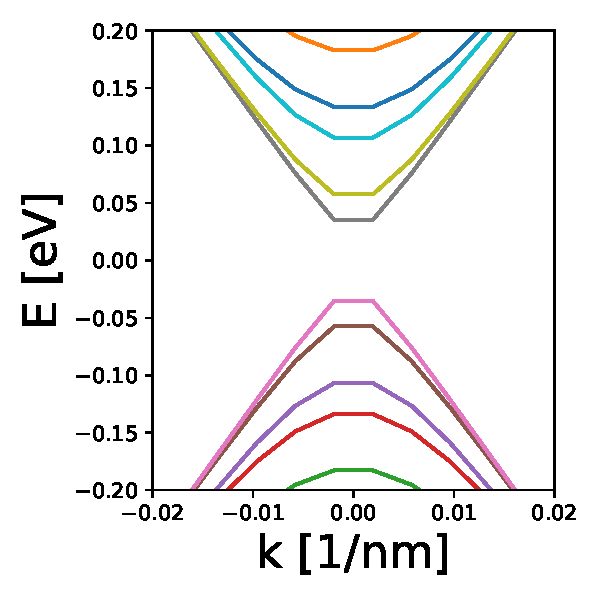
\includegraphics[width=0.77\linewidth]{task1_disp_sf1.pdf}
    \caption{}
    \label{fig:task1-sf1}
\end{subfigure}
\begin{subfigure}{.495\textwidth}
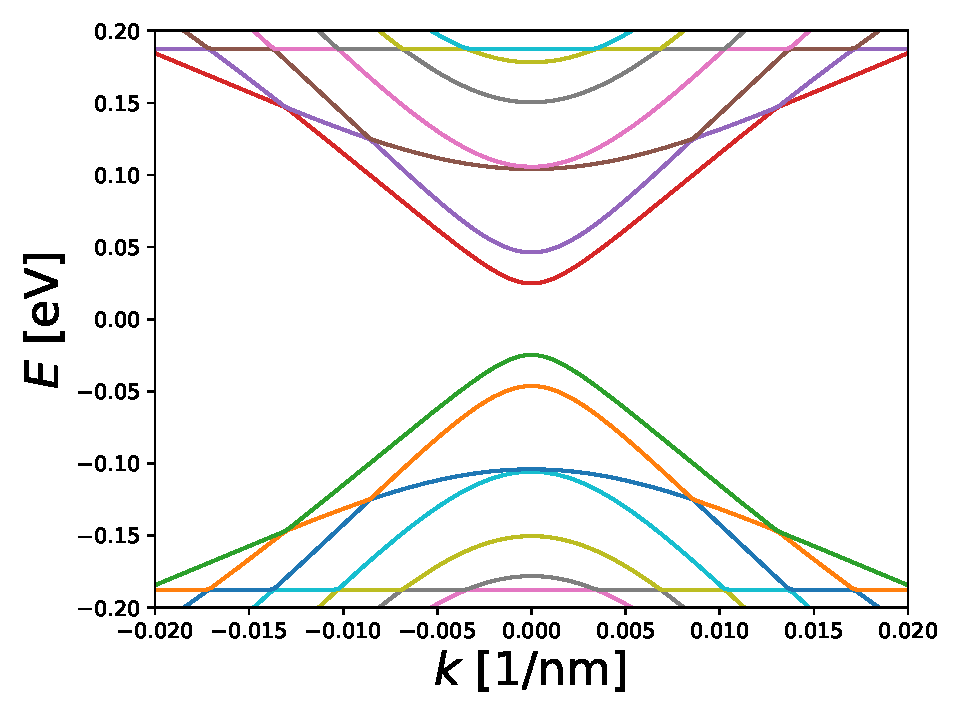
\includegraphics[width=1.\linewidth]{task1_disp_sf16.pdf}
    \caption{}
    \label{fig:task1-sf16}
\end{subfigure}
\caption{Relacja dyspersji (a) dla sf = 1 (b) sf = 16}
\label{fig:task1-sf}
\end{figure}
Dla porównania wyniki zestawiono na jednym rysunku~\ref{fig:task1-both}.
%%%%%%%%%%%%%%%%%%%%%%%%%%%%%%%%%%%%%
\begin{figure}[htp!]
    \centering
    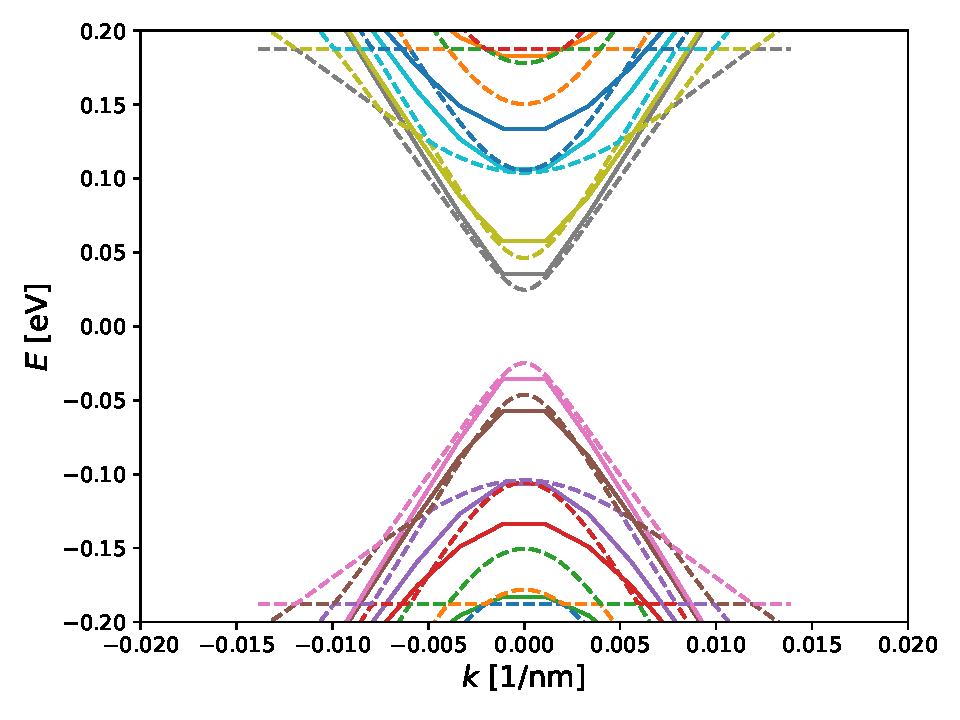
\includegraphics[width=0.65\linewidth]{task1_disp_both.pdf}
    \caption{Porównanie relacji dyspersji: ciągłe krzywe przedstawiają przypadek \texttt{sf=1}, a przerywane - \texttt{sf=16}}
    \label{fig:task1-both}
\end{figure}
%%%%%%%%%%%%%%%%%%%%%%%%%%%%%%%%%%%%%
Zauważmy, że dla niższych energii (na wartość bezwzględną) krzywe się pokrywają.\\
%%%%%%%%%%%%%%%%%%%%%%%%%%%%%%%%%%%%%
\\
Ustaliliśmy  następnie parametry
$$\texttt{y\_min=-79.9, y\_max = 79.9, x\_max = 200, x\_min = -200, Vnp=0.1, B = 1.5}.$$
%%%%%%%%%%%%%%%%%%%%%%%%%%%%%%%%%%%%%
Mapa takiego układu została zapisana na rysunku~\ref{fig:task2-map}.
\begin{figure}
    \centering
    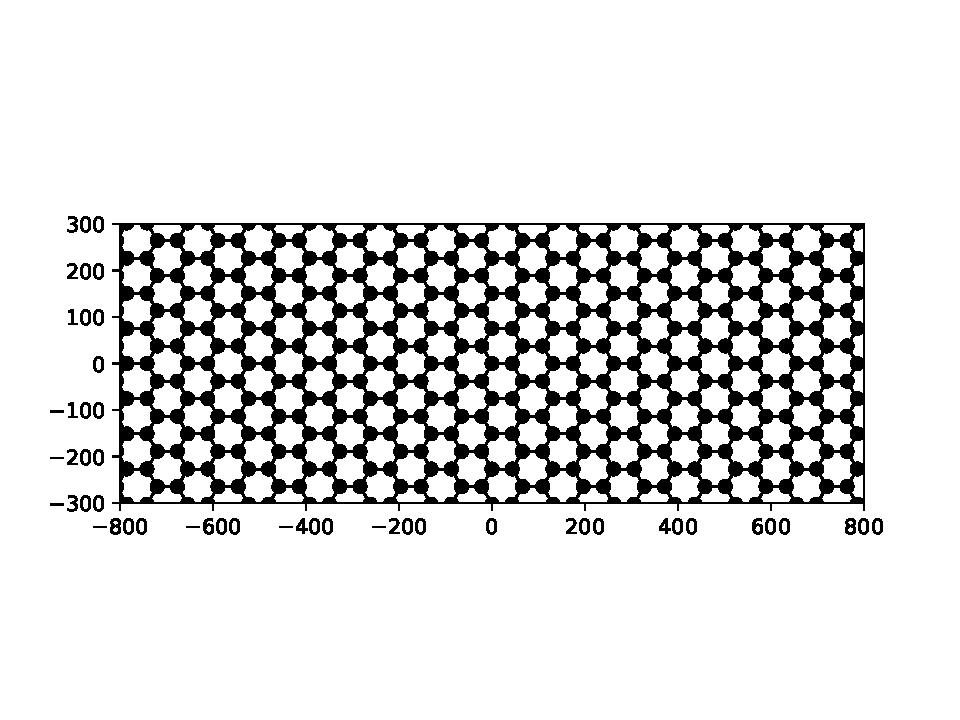
\includegraphics[width=0.7\linewidth]{task2_potential_map.pdf}
    \caption{Mapa układu}
    \label{fig:task2-map}
\end{figure}
%%%%%%%%%%%%%%%%%%%%%%%%%%%%%%%%%%%%%
Zatem ponownie wyznaczyliśmy relację dyspersji (rys.~\ref{fig:task2-B}).
%%%%%%%%%%%%%%%%%%%%%%%%%%%%%%%%%%%%%
\begin{figure}
    \centering
    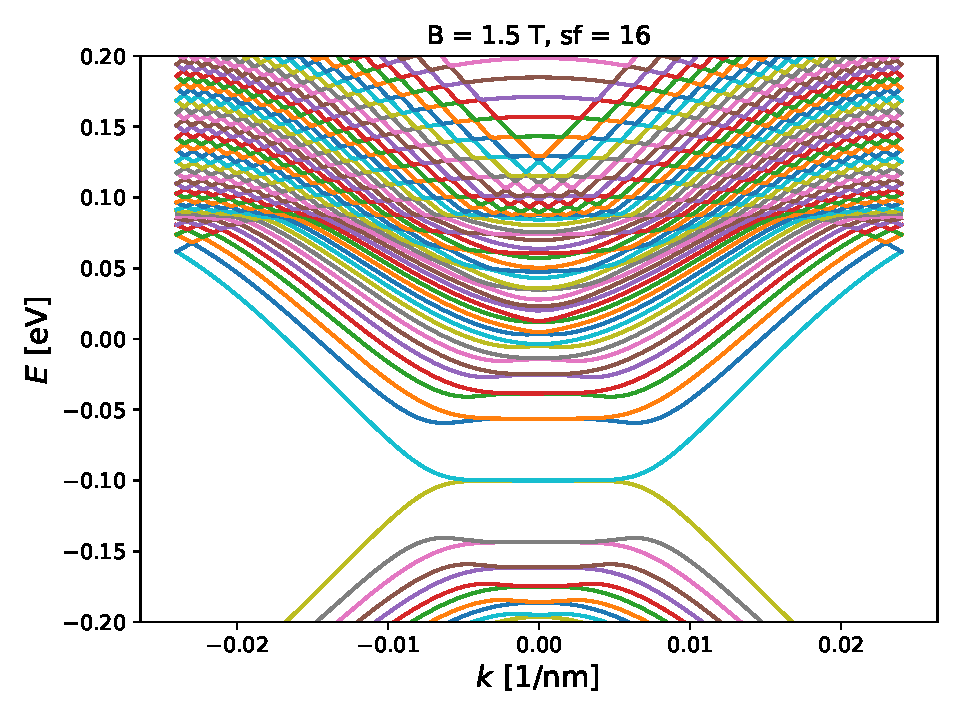
\includegraphics[width=0.5\linewidth]{task2_disp_B1_5.pdf}
    \caption{Relacja dyspersji dla B = 1.5 T, przy sf = 16}
    \label{fig:task2-B}
\end{figure}
%%%%%%%%%%%%%%%%%%%%%%%%%%%%%%%%%%%%%
Możemy wyraźnie zauważyć poziomy Landaua oraz przesunięte spektrum energetyczne o wartość \texttt{Vnp=0.1}~eV.\\
%%%%%%%%%%%%%%%%%%%%%%%%%%%%%%%%%%%%%
\\
Wprowadzając zmienne pole $B$ mogliśmy wyznaczyć wykres konduktancji w funkcji pola $B$.
Wyniki zostały zapisane na rysunku~\ref{fig:task3-cond}.
%%%%%%%%%%%%%%%%%%%%%%%%%%%%%%%%%%%%%
\begin{figure}
    \centering
    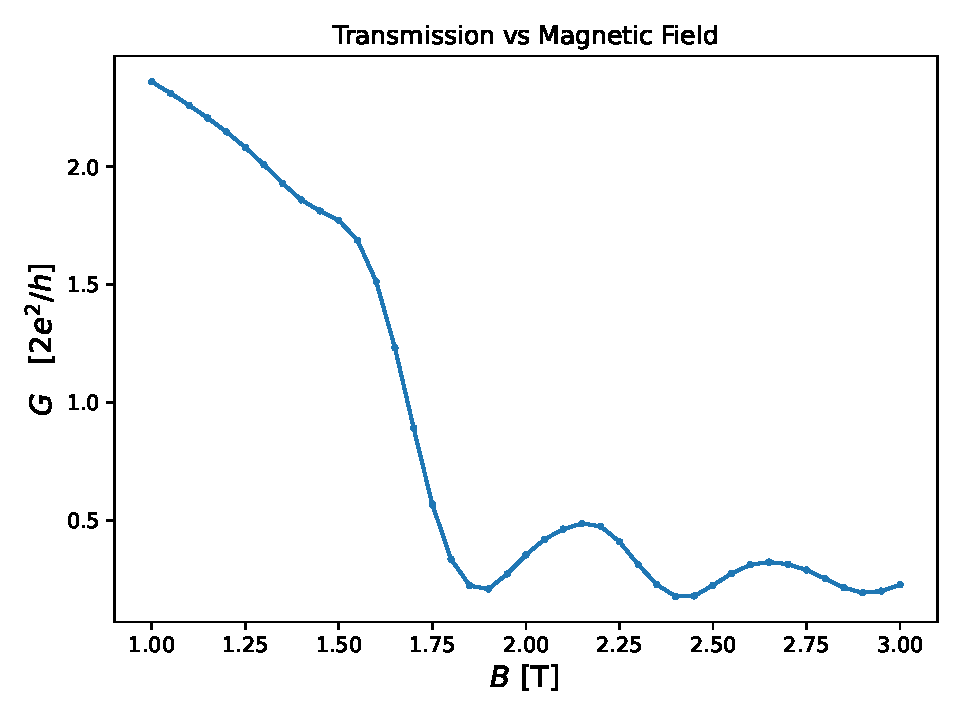
\includegraphics[width=0.5\linewidth]{task3_cond_vs_B.pdf}
    \caption{Przewodność w funkcji pola magnetycznego dla \texttt{Vnp = 0.1} eV}
    \label{fig:task3-cond}
\end{figure}
%%%%%%%%%%%%%%%%%%%%%%%%%%%%%%%%%%%%%
Ostatecznie dla ekstremów lokalnych, które widać na rysunku~\ref{fig:task3-cond} (\texttt{B=1.9, B=2.2, B=2.4}) obliczone zostały mapy prądu na rysunku~\ref{fig:task4-Bs}.
%%%%%%%%%%%%%%%%%%%%%%%%%%%%%%%%%%%%%
\begin{figure}
    \centering
\begin{subfigure}{.495\textwidth}
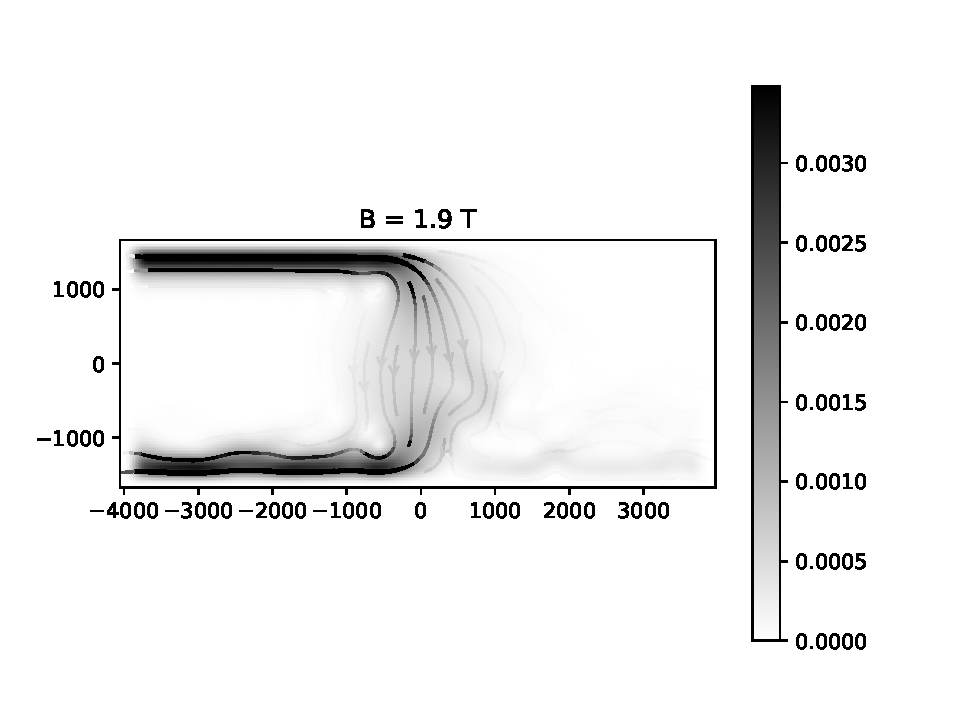
\includegraphics[width=1.\linewidth]{task4_current_B1.9.pdf}
    \caption{}
    \label{fig:task4-B1}
\end{subfigure}
\begin{subfigure}{.495\textwidth}
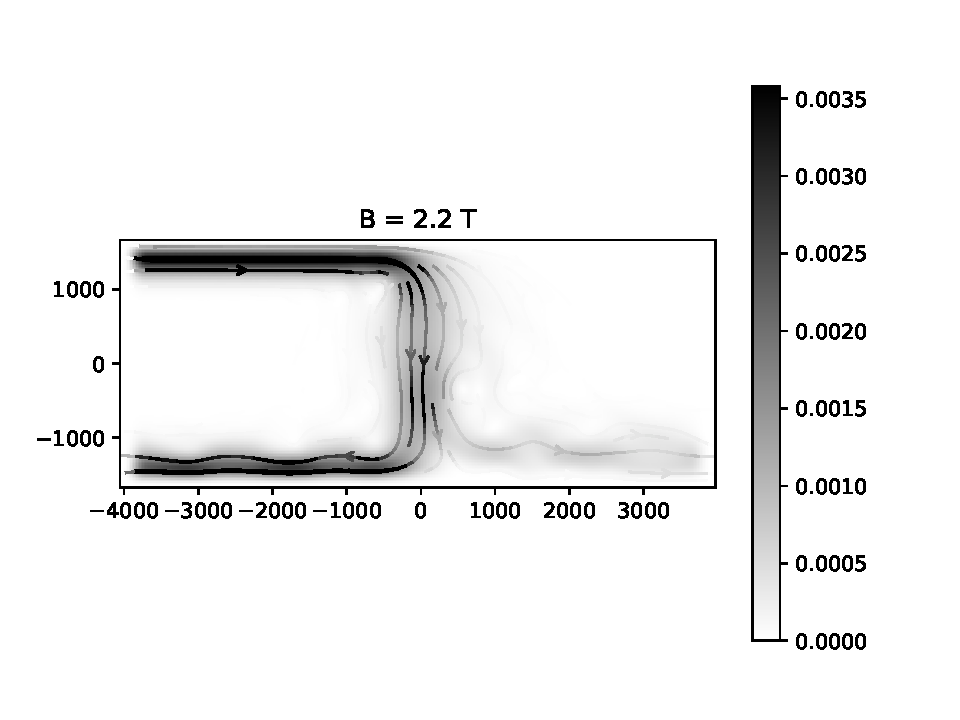
\includegraphics[width=1.\linewidth]{task4_current_B2.2.pdf}
    \caption{}
    \label{fig:task4-B2}
\end{subfigure}
\begin{subfigure}{.495\textwidth}
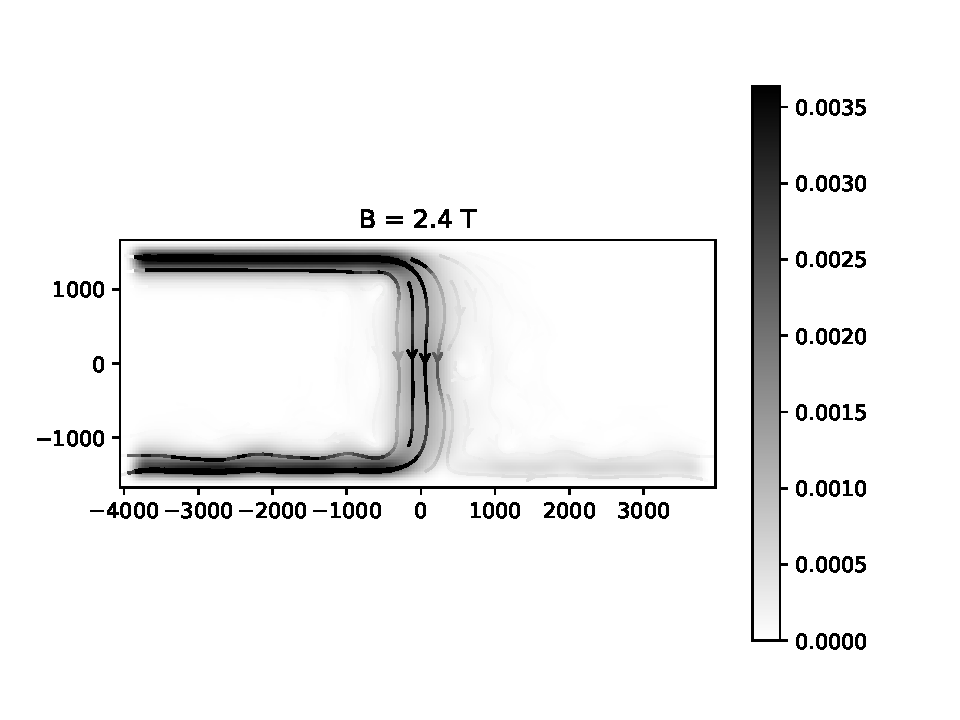
\includegraphics[width=1.\linewidth]{task4_current_B2.4.pdf}
    \caption{}
    \label{fig:task4-B3}
\end{subfigure}
\caption{Mapy prądu przy B odpowiadającego minimum i maksimom G}
\label{fig:task4-Bs}
\end{figure}
%%%%%%%%%%%%%%%%%%%%%%%%%%%%%%%%%%%%%
\section{Podsumowanie}
W ramach ćwiczenia zbadano właściwości układu grafenowego zawierającego złącze typu \textit{p--n} przy użyciu pakietu \texttt{Kwant}. 
Wyznaczono relacje dyspersji dla różnych wartości współczynnika skalowania \texttt{sf}, obserwując ich zgodność przy niskich energiach. \\
\\
Następnie przeanalizowano wpływ pola magnetycznego oraz potencjału złącza na strukturę widma energetycznego, identyfikując poziomy Landaua oraz przesunięcie spektrum energetycznego. 
Obliczono również przewodność w funkcji pola magnetycznego, a dla wybranych jego wartości (w okolicach ekstremów lokalnych przewodności) przedstawiono rozkłady prądu w układzie. 
Wyniki potwierdzają istnienie orbit wężowych w złączu \textit{p--n} w obecności pola magnetycznego.


\end{document}
